\documentclass{beamer}
\usepackage{times}
\usepackage{tikz}
\usepackage{beamerthemesplit} 
\usepackage{tcolorbox}

\title{A Tutorial of White-Box Cryptography \\ Chapter 2 Notions and Definitions}
\author{Zheng Gong\inst{1,2}\\ \url{cis.gong@gmail.com}}
\institute{\inst{1}{School of Computer Science, South China Normal University} \\ \inst{2}{Mobile Applications And Security Engineering Center of Guangdong Province}}

\date{\today}

\begin{document}

\frame
{
 \titlepage
}

\section[Outline]{}
\frame{\tableofcontents}

\section{White-box cryptography}
\frame
{
  \frametitle{The categories of white-box crypto: from crypto side}
  
\begin{itemize}
\setlength{\itemsep}{12pt}
\item symmetric-key
\begin{itemize}

\item \textcolor{red}{block cipher}
\item stream cipher
\item message authentication code
\item pseudorandom generator
\end{itemize}

\item asymmetric-key
\begin{itemize}
\item \textcolor{red}{public-key decryption}
\item \textcolor{red}{signature}
\item multi-party computation
\end{itemize}
\end{itemize}
}

\frame
{
  \frametitle{The categories of white-box crypto: from white-box side}
  
  \begin{itemize}
  \setlength{\itemsep}{12pt}
  \item key escrow resisntance:
  \begin{itemize}
   \setlength{\itemsep}{6pt}
  \item \textcolor{red}{Standalone protection}: N-SPACE, SPNBox
  \item \textcolor{red}{Server-aided protection}: Cloud signature
  \item \textcolor{red}{Complexity hardness}: Chow et al.'s seminal work
  \end{itemize}
  
  \item Code lifting resistance:
  \begin{itemize}
    \setlength{\itemsep}{6pt}
  \item Obfuscation: Space/code/time hardness
  \item Watermarking
  \item Tamper-proofing
  \end{itemize}
   
  \end{itemize}
  
  
}

\section{Recall weak/strong white-box security notions}
\frame
{
\frametitle{Basic security definitions for WBC (Chow \textit{et al.})}
\begin{itemize}
\item In SAC 2002, the security notions have  been informally described for white-box cryptography by Chow \textit{et al.}. First the key recovery problem is informally defined by \textcolor{red}{the weak white-box security}
\end{itemize}


\begin{center}
\begin{tikzpicture}
    \node[anchor=south west,inner sep=0] (image) at (0,0) { 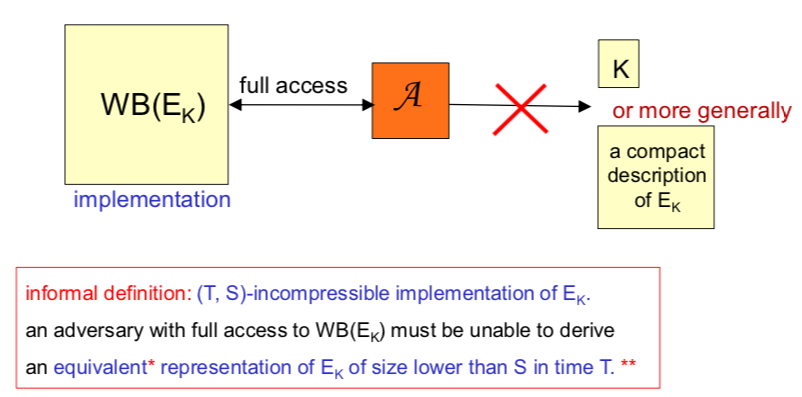
\includegraphics[width=8cm, height=4cm]{./pics/weak_white_box_security.png}};
 
    \begin{scope}[x={(image.south east)},y={(image.north west)}]
        %\draw[help lines,xstep=.1,ystep=.1] (0,0) grid (1,1);
        %\foreach \x in {0,1,...,9} { \node [anchor=north] at (\x/10,0) {0.\x}; }
        %\foreach \y in {0,1,...,9} { \node [anchor=east] at (0,\y/10) {0.\y}; }
        \draw[red, thin, rounded corners] (0.85,0.7) circle (1.2cm);
    \end{scope}
\end{tikzpicture}
\end{center}
}

\frame
{
\frametitle{Basic security definitions for WBC (Biryukov \textit{et al.})}
\begin{itemize}
\item For more general security, \textcolor{red}{the strong white-box security} has been defined by Chow et al.
\end{itemize}

\begin{center}
\begin{tikzpicture}
    \node[anchor=south west,inner sep=0] (image) at (0,0) { 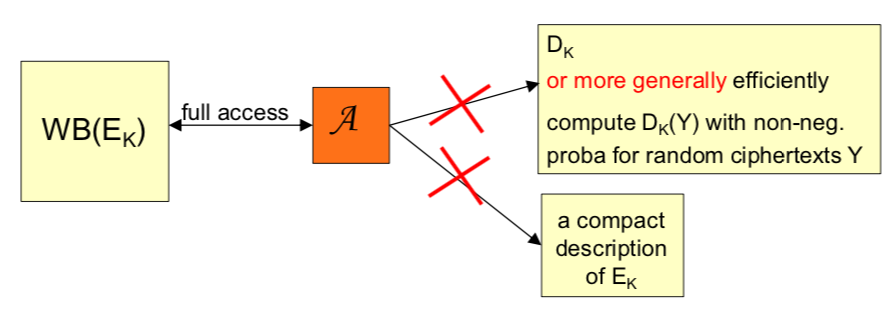
\includegraphics[width=10cm, height=4cm]{./pics/strong_white_box_security.png}};
 
    %\begin{scope}[x={(image.south east)},y={(image.north west)}]
        %\draw[help lines,xstep=.1,ystep=.1] (0,0) grid (1,1);
        %\foreach \x in {0,1,...,9} { \node [anchor=north] at (\x/10,0) {0.\x}; }
        %\foreach \y in {0,1,...,9} { \node [anchor=east] at (0,\y/10) {0.\y}; }
        %\draw[green, ultra thick, rounded corners] (0.24,0.18) rectangle (0.50,0.32);
    %\end{scope}
\end{tikzpicture}
\end{center}
}

\frame
{
\frametitle{Basic security definitions for WBC (3)}
\begin{definition}(\textcolor{red}{Secret key recovery (KR)}). A white-box implementation of a key-instantiated block cipher $E_{k}$ (or $D_{k}$) is called \textit{KR-insecure} if an attacker extracts the secret key $k$ and furthermore has access to the plaintext $P$.
\end{definition}

\begin{definition}
(\textcolor{red}{White-box key recovery (KR)}). A white-box implementation of an encoded version of a key-instantiated block cipher $E_{k}$ (or $D_{k}$) is called \textit{WBKR-insecure} if the attacker extracts the secret key $k$ and the inverse mappings of the applied external encodings.
\end{definition}
}

\frame
{
\frametitle{The shortcomings of traditional crypto model}
\begin{itemize}
 \setlength{\itemsep}{12pt}
 
 \item In the traditional crypto model, e.g., chosen-plaintext/ciphertext attacks, are defined for protecting Kerckhoff's principle. The security goal is just to 
 protect the function (signing, decrypting, etc.)
 
 \item In the white-box security model, attackers already have the ability to use the keyed function, therefore the goal is moved to protect the secrete key or the integrity of the function (not the function itself)!
 
 \item How to define this security model and goal is a challenging work! 
 
\end{itemize}

}

\section{A case study on DRM required white-box security}

\frame
{
\frametitle{Tamper resistance for DRM}

\begin{itemize}
\item Michiels and Gorissen [DRM'07] proposed a method to protect the integrity of software which depends on the correct operation of the white-box implementation of a block cipher.
\item If an attacker modifies the software, the white-box implementation stops decrypting/encrypting properly. 
\begin{tcolorbox}[title=security goal]
\item The proposed method assume that it is the goal of an attacker to modify the protected software without losing the ability to decrypt/encrypt properly.
\end{tcolorbox}
\end{itemize}

}

\frame
{
\frametitle{Tamper resistance with white-box crypto for DRM}

\begin{center}
\begin{tikzpicture}
    \node[anchor=south west,inner sep=0] (image) at (0,0) { 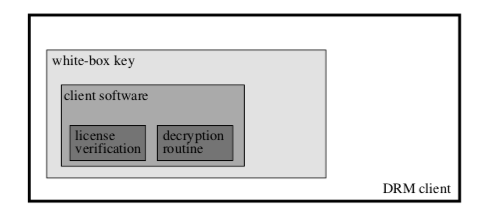
\includegraphics[width=8cm, height=4cm]{./pics/DRM.png}};
 
    %\begin{scope}[x={(image.south east)},y={(image.north west)}]
        %\draw[help lines,xstep=.1,ystep=.1] (0,0) grid (1,1);
        %\foreach \x in {0,1,...,9} { \node [anchor=north] at (\x/10,0) {0.\x}; }
        %\foreach \y in {0,1,...,9} { \node [anchor=east] at (0,\y/10) {0.\y}; }
        %\draw[green, ultra thick, rounded corners] (0.24,0.18) rectangle (0.50,0.32);
    %\end{scope}
\end{tikzpicture}
\end{center}

}

\frame
{
\frametitle{The threat model of Michiels and Gorissen's proposal}
\begin{enumerate}
\setlength{\itemsep}{12pt}
\item A DRM client that is implemented in software and that has to validate conditions in a DRM license before it decrypts the corresponding content. \item The content can be encrypted by AES as this block cipher allows a white-box implementation, which may only be decrypted during a specific time window. 
\item An attacker may try to get around the license by tampering with the program code that verifies the license. 
\item We need not only protect the license verification routine, but also (part of) the software that calls this routine. 
\end{enumerate}
}

\frame
{
\frametitle{The steps of Michiels and Gorissen's proposal}
\begin{enumerate}
\setlength{\itemsep}{12pt}
\item Let B be the binary of the software that we want to protect. 
\item Binary B can be linked and compiled code obtained from higher lever source code, such as C, but it can also be the binary representation of interpreted code, such as byte code in Java. 
\item As binary B is just a string of bits, we can also interpret it as a collection of lookup tables. A code fragment of 1024 bytes can, for instance, be interpreted as a lookup table consisting of 256 rows of 4 bytes.
\end{enumerate}
}

\section{The commercial regulations and administrations}

\frame
{
\frametitle{The published standards}
As a cryptographic product, white-box crypto also has to be regulated and governed by standards.  There are two widely-accepted standards for the security of cryptographic modules:

\begin{itemize}
\setlength{\itemsep}{12pt}
\item FIPS 140-2 (U.S. Standard, internationally accepted)

\item GM/T 0028/0039-2014 (Chinese Standard, learn from FIPS 140-2)
\end{itemize}
}

\frame
{
\frametitle{FIPS 140-2}
In FIPS 140-2, 4 security levels are defined for cryptographic modules to be evaluated
\begin{itemize}
\setlength{\itemsep}{6pt}
\item Level 1:  Use a standard cryptographic algorithm and implement validately

\item Level 2: Achieve Level 1 whilst enforce the role-base authentication on the cryptographic module

\item Level 3: Achieve Level 2 whilst enforce the identity-base authentication on the cryptographic module with physical protection

\item Level 4: Achieve Level 3, intrusion resistance with immediate zeroization, self-test
\end{itemize}

}

\frame
{
\frametitle{FIPS 140-2: Level 1}

\begin{center}
\begin{tikzpicture}
    \node[anchor=south west,inner sep=0] (image) at (0,0) { 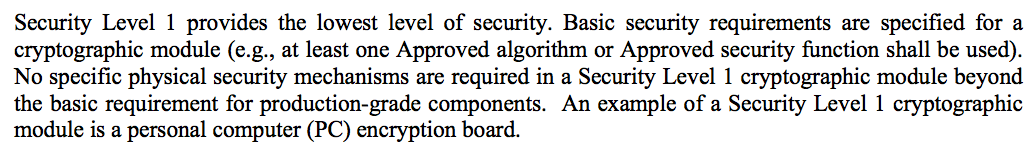
\includegraphics[width=11cm, height=2.1cm]{./pics/Level1.png}};
 
    %\begin{scope}[x={(image.south east)},y={(image.north west)}]
        %\draw[help lines,xstep=.1,ystep=.1] (0,0) grid (1,1);
        %\foreach \x in {0,1,...,9} { \node [anchor=north] at (\x/10,0) {0.\x}; }
        %\foreach \y in {0,1,...,9} { \node [anchor=east] at (0,\y/10) {0.\y}; }
        %\draw[green, ultra thick, rounded corners] (0.24,0.18) rectangle (0.50,0.32);
    %\end{scope}
\end{tikzpicture}
\end{center}

}

\frame
{
\frametitle{FIPS 140-2: Level 2}

\begin{center}
\begin{tikzpicture}
    \node[anchor=south west,inner sep=0] (image) at (0,0) { 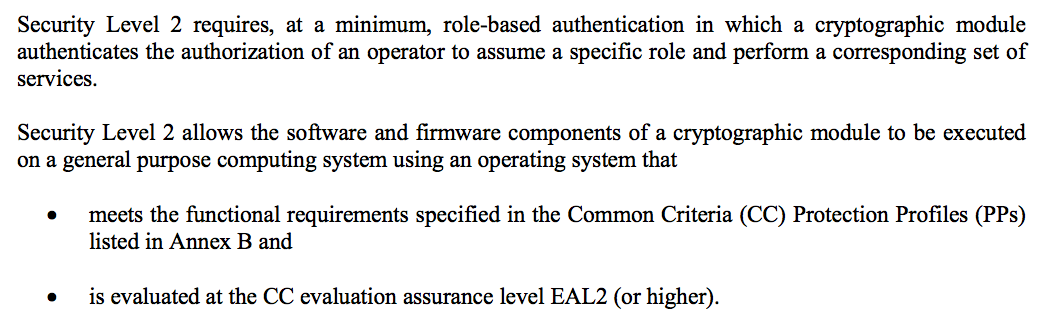
\includegraphics[width=11cm, height=3.4cm]{./pics/Level2.png}};
 
    %\begin{scope}[x={(image.south east)},y={(image.north west)}]
        %\draw[help lines,xstep=.1,ystep=.1] (0,0) grid (1,1);
        %\foreach \x in {0,1,...,9} { \node [anchor=north] at (\x/10,0) {0.\x}; }
        %\foreach \y in {0,1,...,9} { \node [anchor=east] at (0,\y/10) {0.\y}; }
        %\draw[green, ultra thick, rounded corners] (0.24,0.18) rectangle (0.50,0.32);
    %\end{scope}
\end{tikzpicture}
\end{center}

}

\frame
{
\frametitle{FIPS 140-2: Level 3}

\begin{center}
\begin{tikzpicture}
    \node[anchor=south west,inner sep=0] (image) at (0,0) { 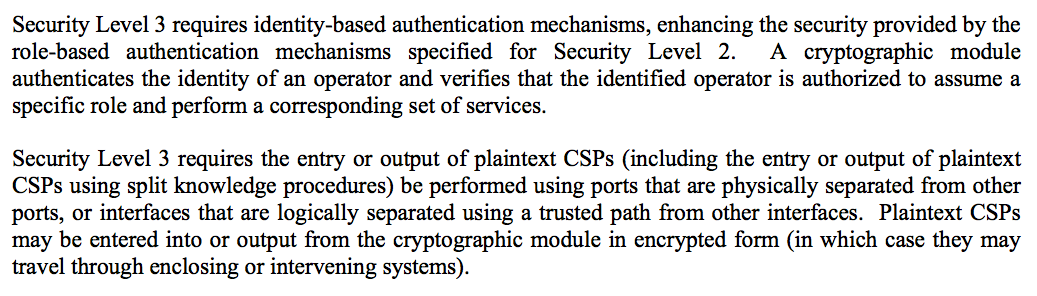
\includegraphics[width=11cm, height=3.4cm]{./pics/Level3.png}};
 
    %\begin{scope}[x={(image.south east)},y={(image.north west)}]
        %\draw[help lines,xstep=.1,ystep=.1] (0,0) grid (1,1);
        %\foreach \x in {0,1,...,9} { \node [anchor=north] at (\x/10,0) {0.\x}; }
        %\foreach \y in {0,1,...,9} { \node [anchor=east] at (0,\y/10) {0.\y}; }
        %\draw[green, ultra thick, rounded corners] (0.24,0.18) rectangle (0.50,0.32);
    %\end{scope}
\end{tikzpicture}
\end{center}

}

\frame
{
\frametitle{FIPS 140-2: Level 4}

\begin{center}
\begin{tikzpicture}
    \node[anchor=south west,inner sep=0] (image) at (0,0) { 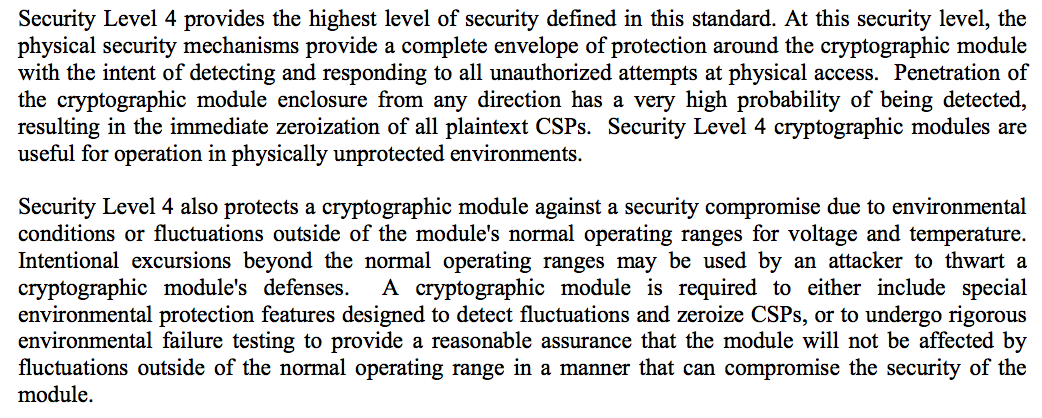
\includegraphics[width=11cm, height=4cm]{./pics/Level4.png}};
 
    %\begin{scope}[x={(image.south east)},y={(image.north west)}]
        %\draw[help lines,xstep=.1,ystep=.1] (0,0) grid (1,1);
        %\foreach \x in {0,1,...,9} { \node [anchor=north] at (\x/10,0) {0.\x}; }
        %\foreach \y in {0,1,...,9} { \node [anchor=east] at (0,\y/10) {0.\y}; }
        %\draw[green, ultra thick, rounded corners] (0.24,0.18) rectangle (0.50,0.32);
    %\end{scope}
\end{tikzpicture}
\end{center}

}

\frame
{
\frametitle{Chinese standard GM/T 0028/0039-2014}
\begin{itemize}
\setlength{\itemsep}{12pt}
\item Also divided into 4 security levels and very similar to FIPS 140-2

\item Add Security Level 2+ and 3+ to fix the gap between software and hardware security assurances.

\item Only for Chinese commercial cryptographic schemes and protocols (SM1/2/3/4/9 series)

\end{itemize}
}


\section{Conclusion}

\frame
{
\frametitle{Conclusion}

\begin{itemize}
\setlength{\itemsep}{12pt}
\item Security notions and definition for \textcolor{red}{precisely} analyze white-box crypto are at very begin

\item Key protection definitions might not suitable in practice for non-key white-box applications, e.g., secure multi-party computation

\item How can we define \textcolor{red}{Strong}/\textcolor{red}{Weak}?
\end{itemize}

}

\frame
{
\begin{center}
\textbf{Thanks for your attentions!}
\end{center}
\begin{center}
\begin{tikzpicture}
    \node[anchor=south west,inner sep=0] (image) at (0,0) { 
\includegraphics[width=4cm, height=4cm]{./pics/WBC_BG.png}};
 
    %\begin{scope}[x={(image.south east)},y={(image.north west)}]
        %\draw[help lines,xstep=.1,ystep=.1] (0,0) grid (1,1);
        %\foreach \x in {0,1,...,9} { \node [anchor=north] at (\x/10,0) {0.\x}; }
        %\foreach \y in {0,1,...,9} { \node [anchor=east] at (0,\y/10) {0.\y}; }
        %\draw[green, ultra thick, rounded corners] (0.24,0.18) rectangle (0.50,0.32);
    %\end{scope}
\end{tikzpicture}

\end{center}
}

\end{document}
